\begin{frame}[t]
  \slideheader{02. DOMAIN ANALYSIS \& EXISTING TOOLS}{Three Existing Paradigms vs. Passage Discovery}

  % Three Equal Visual Product Cards
  \begin{columns}[onlytextwidth, T]
    % Card 1: Splice
    \begin{column}{0.315\textwidth}
      \begin{tcolorbox}[standardcard, top=4pt, bottom=4pt]
        {\small\bfseries\textcolor{textwhite}{Splice}}\par\vspace{0.4mm}
        {\scriptsize\bfseries\textcolor{accentemerald}{Ready-Made Samples}}\par\vspace{1.2mm}
        \centering
        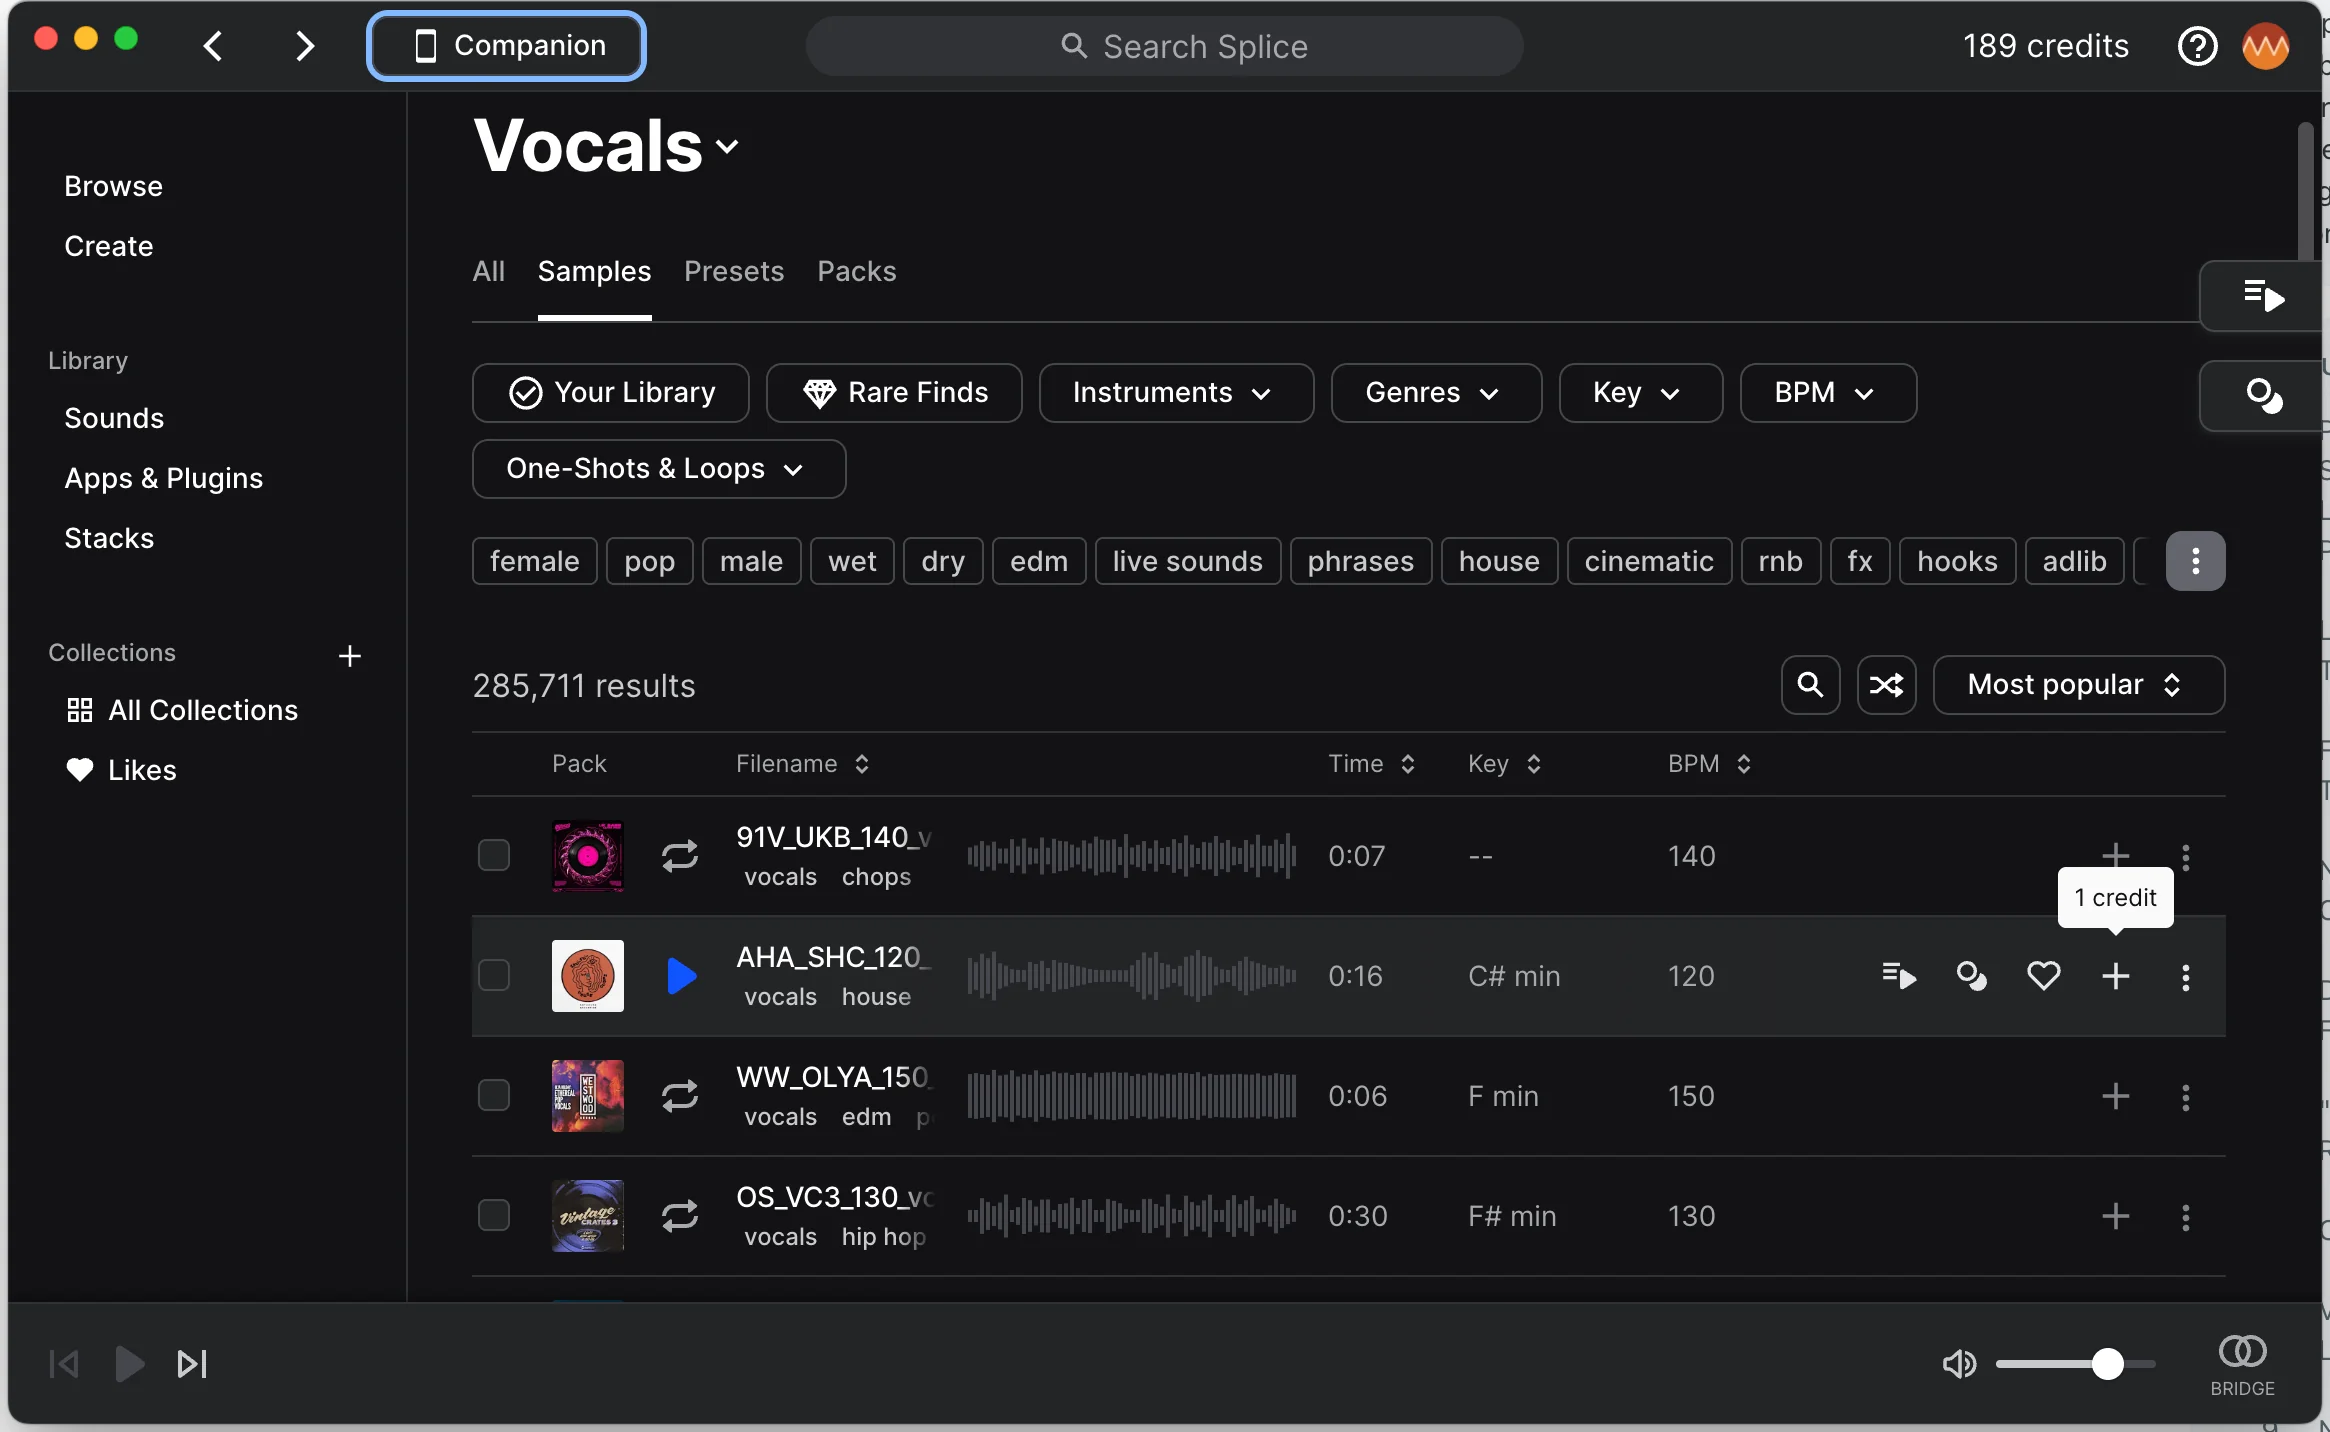
\includegraphics[width=\linewidth, height=2.25cm, keepaspectratio]{images/splice_workflow.png}\par\vspace{1.2mm}
        {\tiny\textcolor{textmuted}{Catalog of pre-cut loops \& one-shots; prepared library workflow.}}
      \end{tcolorbox}
    \end{column}

    % Card 2: Samplette.io
    \begin{column}{0.315\textwidth}
      \begin{tcolorbox}[standardcard, top=4pt, bottom=4pt]
        {\small\bfseries\textcolor{textwhite}{Samplette.io}}\par\vspace{0.4mm}
        {\scriptsize\bfseries\textcolor{accentemerald}{Discover Full Recordings}}\par\vspace{1.2mm}
        \centering
        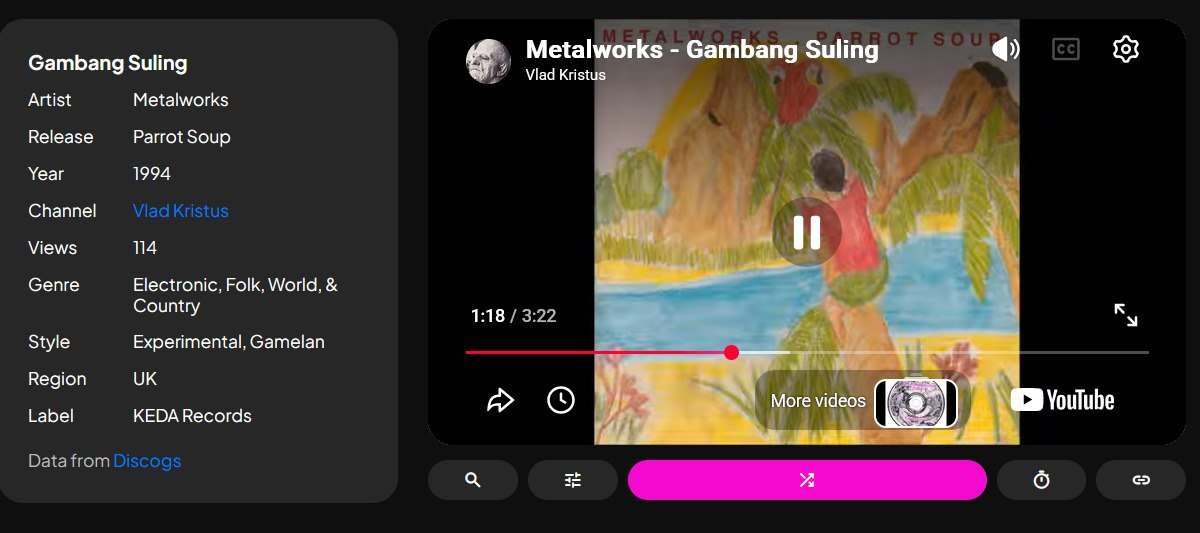
\includegraphics[width=\linewidth, height=2.25cm, keepaspectratio]{images/samplette_work.jpg}\par\vspace{1.2mm}
        {\tiny\textcolor{textmuted}{Randomized YouTube digging via Discogs; whole-track search only.}}
      \end{tcolorbox}
    \end{column}

    % Card 3: Tracklib
    \begin{column}{0.315\textwidth}
      \begin{tcolorbox}[standardcard, top=4pt, bottom=4pt]
        {\small\bfseries\textcolor{textwhite}{Tracklib}}\par\vspace{0.4mm}
        {\scriptsize\bfseries\textcolor{accentemerald}{Licensed Catalog + Tools}}\par\vspace{1.2mm}
        \centering
        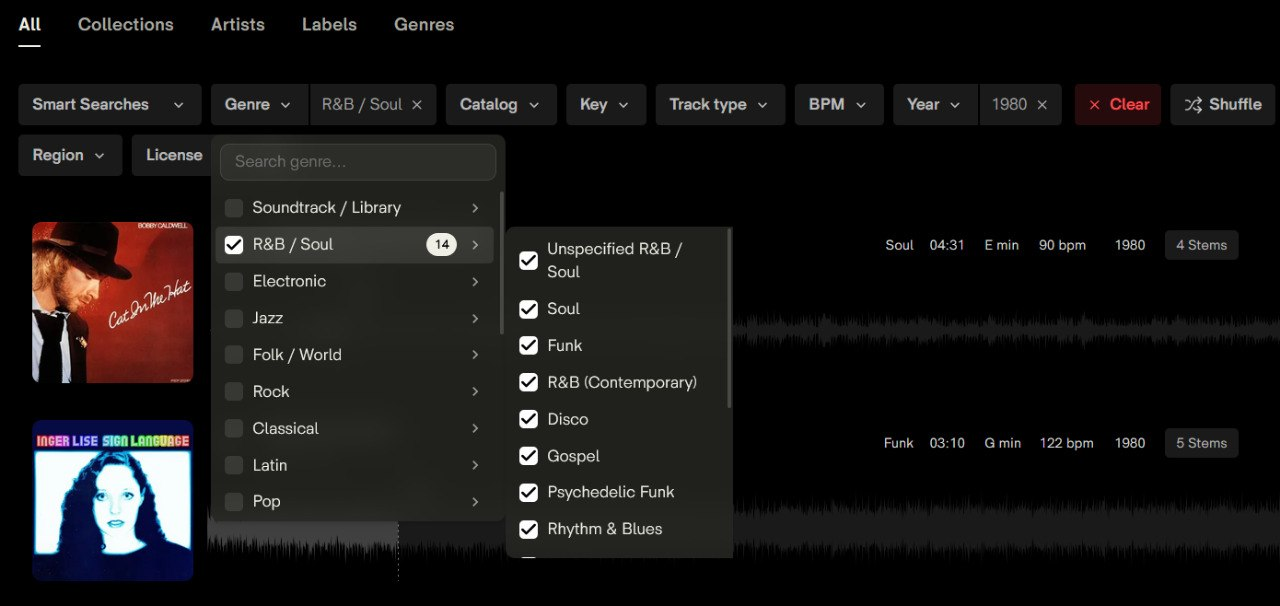
\includegraphics[width=\linewidth, height=2.25cm, keepaspectratio]{images/tracklib_search.jpg}\par\vspace{1.2mm}
        {\tiny\textcolor{textmuted}{Pre-cleared songs with stem isolation and bar-looping tools.}}
      \end{tcolorbox}
    \end{column}
  \end{columns}

  \vspace{2.5mm}

  % Bottom Unified Differentiator
  \begin{tcolorbox}[innercard, left=6pt, right=6pt, top=3.5pt, bottom=3.5pt]
    \centering
    {\small\textbf{\textcolor{accentemerald}{Sample Browser:}} \textcolor{textwhite}{Discover and compare passages across recordings.}}
  \end{tcolorbox}
\end{frame}